%===================================================================================================
\subsection{Sex Work: Population Sizes \& Partner Numbers}\label{model.par.sw}
%---------------------------------------------------------------------------------------------------
\subsubsection{Population Sizes}\label{model.par.sw.size}
Population sizes of all activity groups are modelled as proportions of the total population,
which are assumed to remain roughly constant,
although individuals can move between groups (see \sref{model.par.turn.act}),
and disproportionate mortality due to HIV between groups
may cause higher risk groups to shrink over time.
%---------------------------------------------------------------------------------------------------
\paragraph{Female Sex Workers}
The proportion of women who report sex work in national demographic and health surveys
is generally considered unreliable due to social desirability bias,
particularly if the survey is face-to-face and household-based
\cite{Konings1995,Gregson2002,Gregson2004,Lowndes2012,Behanzin2013}.
Therefore, FSW population size estimates require
targeted surveys and unique methodologies \cite{UNAIDS2010kps,Abdul-Quader2014}.
In both \cite{EswKP2014} and \cite{EswIBBS2022}, the Swati FSW population size
was estimated using a combination of
unique object method, service multiplier method, prior survey participation,
and network scale-up method (NSUM) \cite{UNAIDS2010kps}.
In 2011 \cite{EswKP2014}, regional FSW population size estimates
ranged from 0.7\% to 6.5\% of all women,
with overall population-weighted mean across regions of 2.9\%;
in 2021 \cite{EswIBBS2022}, the mean (95\%~CI) estimates were 2.43~(1.17,~5.02)\%.
To reflect this uncertainty in the model, a BAB distribution was fitted
such that 95\% of the probability fell between 0.7\% and 6.5\%,
and used as the prior distribution for the proportion of women who are FSW:
$P_{s_{1}i_{34}} / P_{s_{1}}$.
Then, following the analysis in \sref{model.par.fsw},
the proportion of all FSW in the higher risk FSW group was fixed at 20\%,
and likewise the lower risk group at 80\%.
%---------------------------------------------------------------------------------------------------
\paragraph{Clients of FSW}
Similar to FSW, household-based surveys are not considered reliable data sources
for estimating the population size of clients of FSW \cite{Behanzin2013}.
However, few surveys are designed to reach clients of FSW,
and no direct estimates of FSW size exist for Eswatini.
So, I use a common approach for inferring the FSW client size \cite{Cote2004},
similar to the ``multiplier method'' \cite{Morison2001}.
Given the FSW population proportion $P_{s_{1}i_{34}}$,
the number of average yearly new and regular sex work clients per FSW $Q_{p_{34}s_{1}i_{34}}$,
the frequency of sex per partnership-year $F_{p_{34}}$, and
the total number of yearly commercial sex acts per client year $Q_{p_{34}s_{2}i_{34}}\,F_{p_{34}}$,
the total client population $P_{s_{2}i_{34}}$ is defined as:
\begin{equation}
  {\textstyle\sum_{i}} P_{s_{2}i_{34}} =
  \frac{\sum_{pi} P_{s_{1}i}\,Q_{p_{34}s_{1}i_{34}}\,F_{p_{34}}}
       {\sum_{pi}             Q_{p_{34}s_{2}i_{34}}\,F_{p_{34}}}
  \label{eq:model.fsw.cli.tot}
\end{equation}
Then, as with FSW, the proportion of total clients in the higher risk client group
is defined as 20\% of all clients, and likewise for the lower risk group at 80\%.
Using $Q_{p_{34}s_{1}i_{34}}$, $Q_{p_{34}s_{2}i_{34}}$, and $F_{p_{34}}$
as defined below in \sref{model.par.sw.part}, the client population size $P_{s_{2}i_{34}}$
estimated by this method was 13.1~(2.1,~38.5)\% of men. % TODO: double check
%---------------------------------------------------------------------------------------------------
\subsubsection{Sex Work Partnerships}\label{model.par.sw.part}
%---------------------------------------------------------------------------------------------------
\paragraph{Female Sex Workers}
Table~\ref{tab:fsw.ratios} summarizes
the numbers of new and regular clients \emph{per month} reported by Swati FSW,
stratified by higher \vs lower risk per the analysis in \sref{model.par.fsw.fac}.
In general, the numbers of partners ``$C$'' reported
for a given recall period $\gamma$ (\eg 1 month)
do not directly inform a partnership formation rate $Q$ nor a number of concurrent partners $K$
(see \sref{app.model.math.qp});
rather, under certain assumptions, $Q$ and $K$ can be defined as:
\begin{alignat}{1}
  Q &= \frac{C}{\gamma+\delta} \label{eq:C2Q}\\
  K &= \frac{C\delta}{\gamma+\delta} = Q\delta \label{eq:C2K}
\end{alignat}
The choice of force of infection model (see Chapter~\ref{foi})
will determine whether $Q$ or $K$ is used.
Moreover, based on the survey questions,%
\footnote{The survey questions were: \shortquote{In the last 30 days,
  how many (new/regular) clients have you had sex with?}, or similar.}
it's not clear whether these reported partner numbers $C$
represent the numbers of unique men or unique client visits.
\par
I assumed that all \emph{new} clients were one-off visits;
thus the reported partner numbers effectively represented
$1/12$th of the total numbers of yearly partnerships $Q_{p_{3}}$.
As such, I sampled the yearly rate of new sex work partnerships among lower risk FSW
from a gamma distribution with mean (95\%~CI) as 4.1~(2.5,~6.0) $\times$ 12,
and the \emph{relative} rate among higher risk FSW from 2.0~(1.6,~2.5).
Since each partnership is assumed to include only one sex act,
the partnership duration $\delta_{p_{3}}$, frequency of sex $F_{p_{3}}$,
and number of concurrent partnerships $K_{p_{3}}$ are ill-defined,
but can be defined for convenience as
$\delta_{p_{3}} = 1/12$ (years), $F_{p_{3}} = 12$ (per year),
and $K_{p_{3}} = Q_{p_{3}} / 12$ (per year).
\par
For \emph{regular} sex work partnerships, uncertainties remain regarding
partnership duration $\delta_{p_{4}}$ (see \sref{model.par.sex.dur}),
frequency of sex per month $F_{p_{4}}/12$, and
survey responses $C$ reflecting unique clients or total client visits per month.
If $C$ reflects the numbers of unique clients, then
$Q_{p_{4}s_{1}i_{34}}$ can be defined via \eqref{eq:C2Q} using $C$ directly;
whereas if $C$ reflects the numbers of unique visits, then
$Q_{p_{4}s_{1}i_{34}}$ should be defined using $C/(F_{p_{4}}/12)$.
I assumed that $\rho = 2/3$ of respondents interpreted the question as in the former case,
and $1-\rho = 1/3$ as in the latter, such that:
\begin{equation}\label{eq:C.swr}
  C' = \rho\,C + (1-\rho)\,C/(F_{p_{4}}/12)
\end{equation}
Taking $F_{p_{4}}/12 = 2$ as the prior mean from \sref{model.par.sex.freq},
\eqref{eq:C.swr} simplifies to $C' = \frac{5}{6}\,C$.
Then, sampling $C_{p_{4}s_{1}i_{3}}$
from a gamma distribution with mean (95\%~CI) 8.4~(6.0,~11.0) from Table~\ref{tab:fsw.ratios},
and $\delta_{p_{4}}$ as specified in \sref{model.par.sex.dur},
I defined $Q_{p_{4}s_{1}i_{3}}$ and $K_{p_{4}s_{1}i_{3}}$
via \eqref{eq:C2Q} using $C'_{p_{4}s_{1}i_{3}}$ and $\gamma = 1/12$ year.
% TODO: summarize distributions: Q, K, KF
For higher risk FSW, I sampled the \emph{relative} number/rate of regular clients from
1.5~(1.3,~1.7) (Table~\ref{tab:fsw.ratios}) as before.
%---------------------------------------------------------------------------------------------------
\paragraph{Clients}
For Sub-Saharan African clients of FSW, data on
the number of unique FSW visited and the frequency of sex is sparse.
Among 64 clients in Kenya,
the median number of sex work visits per week was 1.3 (68 per year);
most clients (68\%) had 1--3 regular FSW partners simultaneously, and
visited 0--3 new FSW per year \cite{Voeten2002}.
Among 261 truck drivers at sex work hotspots in Uganda,
the mean number of sexual partners was
7.4 in the past 30 days and 44.7 in the past year \cite{Matovu2012}.
\citet{Johnson2017} modelled yearly sex work visits among South African clients of FSW as
gamma-distributed with age over 10, peaking at 64 visits per year for clients aged 37.
To reflect these data, I specified clients overall to have
mean (95\%~CI) 60~(35,~90) sex acts with FSW per year
($K_{p_{34}s_{2}i_{34}}\,F_{p_{34}}/12$, gamma prior).
Then, the yearly sex acts among lower and higher risk clients are defined such that
higher risk have 2.0~(1.6,~2.5) times the number risk.
Finally, since the distribution of sex acts between new \vs regular sex work partnerships
must match that among FSW, the specific values of $K_{p_{34}s_{2}i_{34}}$
were computed automatically.
% TODO: summarize distributions: Q, K, KF
See \sref{model.par.nsw.sw} for numbers of main/spousal and casual partnerships
among FSW and clients.
%===================================================================================================
\subsection{Non-Sex Work: Group Sizes \& Partner Numbers}\label{model.par.nsw}
%---------------------------------------------------------------------------------------------------
\subsubsection{Reported Partner Numbers}\label{model.par.nsw.report}
% TODO: Cockcroft2010 (!)
The 2006-07 DHS \cite{SDHS2006}, 2011 SHIMS \cite{SHIMS1}, and 2016-17 SHIMS2 \cite{SHIMS2} surveys
provide the numbers of respondents who reported 2+ partners in the past 12 months (p12m):
13.5, 18.2, 14.5\% among men, and 1.6, 3.8, 4.1\% among women, respectively.%
\footnote{From
  Tables~14.7.1 and 14.7.2 (ages 15-49) in \cite{SDHS2006},
  Table~3 (ages 18-49) in \cite{SHIMS1},
  Table~15.3.A (ages 15+) in \cite{SHIMS2},
  with manual adjustment for survey skip patterns in \cite{SDHS2006,SHIMS2}.}
However, these data do not provide information on the types of partners reported
--- \ie those reporting 1 partner in p12m
are not necessarily in a main/spousal (vs casual) partnership,
and neither are those reporting 2+ partners in p12m.
Moreover, such reports are likely substantially biased by
social desirability bias due to the face-to-face interview format
\cite{Konings1995,Plummer2004,Gregson2004,Behanzin2013}.
\par
Regarding the types of partnerships reported.
Both the 2006 DHS \cite[Tables 14.6.1 and 14.6.2]{SDHS2006}
and 2016-17 SHIMS \cite[Tables 15.4.A and 15.4.B]{SHIMS2}
summarize the numbers of women and men by partners in p12m \emph{and} by marital/union status,
although summaries are stratified by each factor separately, not jointly.
However, making the following assumptions,
I estimated the jointly-stratified proportions of individuals.
Let $W_{2+}$, $W_{1}$, and $W_{0}$ denote women reporting 2+, 1, and 0 partners, respectively,
and likewise with $M_{2+}$, $M_{1}$, $M_{0}$ for men (all partners reflect p12m).%
\footnote{Regarding notation in this section,
  $W_{2+} = P_{s_{1}i_{234}} / P_{s_{1}}$,
  $W_{1} + W_{0} = P_{s_{1}i_{1}} / P_{s_{1}}$, and likewise for men ($M$, $s = 2$).}
The assumptions were:
\begin{itemize}
  \item $W_{2+}$ included all women in non-polygynous unions (married or cohabiting)
  reporting sex with a ``casual'' (non-marital, non-cohabiting) partner
  \item $M_{2+}$ included all men in polygynous unions,
  plus all men in non-polygynous unions reporting sex with a casual partner
  \item the remaining $W_{2+}$ and $M_{2+}$ formed only casual partnerships
  \item all women and men in non-polygynous unions
  reporting no sex with a casual partner reported 1 partner ($W_{1}$ and $M_{1}$)
  \item the remaining $W_{1}$ and $M_{1}$ formed only casual partnerships
\end{itemize}
Figure~\ref{fig:Cwp} illustrates the resulting
proportions of women and men in each union/partners in p12m stratum
in 2006-07 \sfref{fig:Cwp.2006} and 2016-17 \sfref{fig:Cwp.2016}.
\begin{figure}
  \centering
  \begin{subfigure}{0.7\linewidth}
    \centering
    \includegraphics[width=\linewidth]{Cwp.2006}
    \caption{2006-07 \cite{SDHS2006}}
    \label{fig:Cwp.2006}
  \end{subfigure}
  \begin{subfigure}{0.7\linewidth}
    \centering
    \includegraphics[width=\linewidth]{Cwp.2016}
    \caption{2016 \cite{SHIMS2}}
    \label{fig:Cwp.2016}
  \end{subfigure}
  \begin{subfigure}{0.7\linewidth}
    \centering
    \includegraphics[width=\linewidth]{Cwp.adj}
    \caption{Adjusted (mean)}
    \label{fig:Cwp.adj}
  \end{subfigure}
  \caption{Reported proportions of women and men aged 15--49,
    stratified by union status and numbers of partners in the past 12 months}
  \label{fig:Cwp}
\end{figure}
%---------------------------------------------------------------------------------------------------
\paragraph{Reporting Bias}
Next, I consider the issue of reporting bias.
$M_{2+}$ is consistently much greater than $W_{2+}$.
This difference is common in surveys \cite{Todd2009,Higgins2010}, and could be explained by either:
(a) a small number of women with many partners,
such as FSW, who may also not be reached by the survey,
or who may not fully report partner numbers;
(b) over-reporting of partnerships by men; or
(c) under-reporting of partnerships by women.
Further stratification of women reporting 2+ partners in \cite[Table~14.7.1]{SDHS2006}
revealed that 94\% reported exactly 2 whereas 6\% reported 3+,
suggesting that explanation (a) is less likely unless
women with 3+ partners are under-reported or indeed missing from the survey.
\par
\citet{Gregson2002} (Zimbabwe), \citet{Nnko2004} (Tanzania) and \citet{Clark2011} (Kenya)
explored explanations (b) and (c) through measures of consistency; their results suggested that
under-reporting of non-spousal partnerships by women (c) was more likely,
perhaps due to social norms and pressures;
such norms in Eswatini are explored in \cite{Ruark2014,Fielding-Miller2016,Ruark2019,Pulerwitz2021}.
In fact, a review comparing computer-based tools \vs face-to-face interviews
for surveying sexual behaviour \cite{Langhaug2010} found that
\emph{both} women and men may under-report sexual partners, but women more so.
A notable study in Benin \cite{Behanzin2013} found that
7 times as many married women (21 \vs 3\%) and 3 times as many married men (53 \vs 18\%)
reported any extramarital sex in p12m
in a surveys via anonymous polling booth \vs face-to-face interview.
Similarly, 5 times as many unmarried women (13.5 \vs 2.8\%) reported
exchanging sex for money, gifts or favours in p12m, while
4 times as many unmarried men (62 \vs 14\%) reported non-transactional sex with a women in p12m.
Such findings were similar to those from Zimbabwe (1990s) \cite{Gregson2002}.
%---------------------------------------------------------------------------------------------------
\subsubsection{Bias Adjustment: Approach}\label{model.par.nsw.bias}
Reflecting these potential reporting biases
and qualitative insights from \cite{Ruark2014,Fielding-Miller2016,Ruark2019,Pulerwitz2021},
I modelled the ``true'' proportions of Swati women and men
in each union/partners in p12m stratum as follows.
Let $W_{s1}$ and $W_{u1}$ denote sub-proportions of $W_{1}$ who are single and in a union, respectively,
and likewise for $W_{s2+}$, $W_{u2+}$, $M_{s1}$, $M_{u1}$, $M_{s2+}$, and $M_{u2+}$.
Further, let $W_{s1}$ denote the reported proportion of women (average of 2006-07 and 2016-17),
\vs $W'_{s1}$ denoting the ``true'' (adjusted) proportion.
I assumed that a faction of $W_{0}$ belongs in $W'_{s1}$
--- \ie a fraction of women reporting 0 partners in p12m truly had 1 casual (non-main/spousal) partner.
I modelled this relationship through an odds ratio $\varphi_{W,s1:0}$,
which is roughly equivalent in interpretation to
the proportion ratios estimated by \citet{Behanzin2013}:%
\footnote{Odds ratios ensure no proportions become greater than one or negative.}
\begin{equation}\label{eq:Cwp.or}
  \varphi_{Ws1:0} = \frac{W'_{s1}}{W'_{0}} \bigg/ \frac{W_{s1}}{W_{0}}
\end{equation}
I defined similar odds ratios $\varphi_{Ws2+:s1}$, $\varphi_{Wu2+:u1}$,
$\varphi_{Wu1:0}$, $\varphi_{Wu1:s1}$, and $\varphi_{Wu2+:s2+}$, and likewise for men.
The corresponding transitions of women from reported to ``true'' strata
are illustrated in Figure~\ref{fig:model.nsw.adj}.
To resolve the adjusted values $W'$ then requires
solving the (nonlinear) system of 6 equations corresponding to the 6 odds ratios $\varphi$,
subject to $\sum_i W'_i = 1$ and $0 \le W'_i < 1$.
An exact solution is not guaranteed,
but the sum squared error from all equations can be minimized.
The odds ratios $\varphi$ were then defined as follows, including sampling distributions.
\begin{figure}
  \centering
  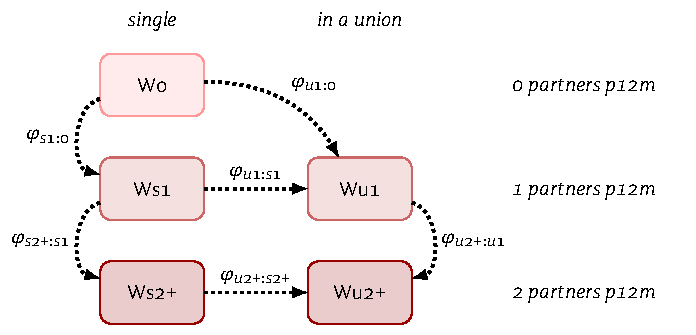
\includegraphics[scale=.8]{diag.nsw.adj}
  \caption{Illustration of how women (and equivalently men)
    are reallocated between union/partners in p12m strata
    based on odds ratios $\varphi$}
  \label{fig:model.nsw.adj}
  \floatfoot{\raggedright
    p12m: within the past 12 months
    W0: 0 partners in p12m;
    Ws1: single (not married/cohabiting) and 1 partner in p12m;
    Wu1: in a union (married/cohabiting) and 2+ partners in p12m;
    Ws2+: single and 2+ partners in p12m;
    Wu2+: in a union and 2+ partners in p12m.
    $\varphi$: odds of truly being in the second (arrowhead) vs first (tail) group.}
\end{figure}
%---------------------------------------------------------------------------------------------------
\paragraph{Union Status}
I assumed that under-reporting of main/spousal partnerships was minimal,
but that some ``main'' partnerships may not be captured in
the definition ``married/cohabiting'' from \cite{SDHS2006,SHIMS2};
thus $\varphi_{u1:0}$, $\varphi_{u1:s1}$, and $\varphi_{u2+:s2+}$
would be small but greater than 1
(horizontal transitions in Figure~\ref{fig:model.nsw.adj}).
Moreover, based on the median age of marriage, 23--29 \cite{SDHS2006},
approximately half of respondents aged 15--49 would have been married,
whereas only 28--39\% of women and men reported being in a union
(Figure~\ref{fig:Cwp.2006}~and~\ref{fig:Cwp.2016}),
although some marriages end in divorce/widowing \cite{SDHS2006}.
Thus, I sampled each of $\varphi_{u1:0}$, $\varphi_{u1:s1}$, and $\varphi_{u2+:s2+}$
from $1+\opname{Gamma}(\alpha,\beta=1)$
with $\alpha=.5$ for women and $\alpha=.3$ for men,
yielding mean (95\%~CI): 1.50~(1.00,~3.51) and 1.30~(1.00,~2.90), respectively.
%---------------------------------------------------------------------------------------------------
\paragraph{Partner Numbers}
Next, I defined $\varphi_{s1:0}$, $\varphi_{s2+:s1}$, and $\varphi_{u2+:u1}$ as follows
(vertial transitions in Figure~\ref{fig:model.nsw.adj}).
The median age of first sex in Eswatini was
approximately 18 for women and 19.5 for men \cite{SDHS2006}.
Thus, the 31--36\% of women and 34--41\% of men aged 15--49 reporting no partners in p12m
(Figure~\ref{fig:Cwp.2006}~and~\ref{fig:Cwp.2016}) is likely overestimated,
although some individuals may be abstinent in p12m following sexual debut.
I assumed that women had 3 and men had 2 times the odds of
actually having 1 casual partner in p12m while reporting no partners.
Thus, I sampled $\varphi_{s1:0}$ from $1+\opname{Gamma}(\alpha,\beta=1)$
with $\alpha=2$ for women and $\alpha=1$ for men,
yielding mean (95\%~CI): 3.00~(1.24,~6.57) and 2.00~(1.03,~4.69), respectively.
Drawing on \cite{Behanzin2013}, I assumed that ``single'' women and men (not married/cohabiting)
were less likely to report multiple partners in p12m, but women more so.
Thus, I sampled $\varphi_{s2+:s1}$ from $1+\opname{Gamma}(\alpha,\beta=1)$
with $\alpha=4$ for women and $\alpha=1$ for men,
yielding 5.00~(2.09,~9.77) and 2.00~(1.03,~4.69).
I made a similar assumption about married/cohabiting women and men,
with the same odds for men, but even greater odds of non-reporting among women.
I sampled $\varphi_{u2+:u1}$ from $1+\opname{Gamma}(\alpha,\beta=1)$
with $\alpha=6$ for women and $\alpha=1$ for men,
yielding 7.00~(3.20,~12.67) and 2.00~(1.03,~4.69).
%---------------------------------------------------------------------------------------------------
\subsubsection{Bias Adjustment: Resulting Group Sizes \& Partner Numbers}\label{model.par.nsw.res}
The mean resulting adjusted proportions $W'$ and $M'$
from solving the system with the assumed odds ratios $\varphi$
are illustrated in Figure~\ref{fig:Cwp.adj}, which can be compared to
the reported proportions in \sfref{fig:Cwp.2006}~and~\sfref{fig:Cwp.2016}.
Figure~\ref{fig:Cwp.adj.dens} also illustrates the empiric density distributions
for each element $W'_{i}$ and $M'_{i}$.
Numerically, the mean (95\%~CI) estimates were:
\begin{itemize}
  \item $W'_{0} = 17~(9,~27)$\% of women and $M'_{0} = 25~(13,~35)\%$ of men had 0 partners in p12m
  \item $W'_{1} = 66~(57,~75)$\% of women and $M'_{1} = 49~(37,~61)\%$ of men had 1 partners in p12m
  \item $W'_{2+} = 17~(10,~27)$\% of women and $M'_{2+} = 26~(15,~44)$\% of men had 2+ partners in p12m
  \item $W'_{u1} / W'_{01} = 38~(21,57)$\% women and $M'_{u1} / M'_{01} = 35~(23,~50)$\% men
    with 0--1 partners in p12m were in a main/spousal partnership
  \item $W'_{s1} / W'_{01} = 41~(19,65)$\% women and $M'_{s1} / M'_{01} = 31~(15,~55)$\% men
    with 0--1 partners in p12m were in a single casual partnership
  \item $W'_{u2+} / W'_{2+} = 32~(9,55)$\% women and $M'_{u2+} / M'_{2+} = 38~(13,~62)$\% men
    with 2+ partners in p12m were in a main/spousal partnership,
    and the rest had only casual partnerships.
\end{itemize}
%---------------------------------------------------------------------------------------------------
\paragraph{Group Sizes}
From these results, I defined the sizes of the modelled lower and medium activity groups,
and the average numbers of main/spousal partnerships per person.
I assumed that $W'_{2+}$ and $M'_{2+}$ included FSW and client population sizes, respectively
(see \sref{model.par.sw.size}).
Thus, the populations size of medium activity women was defined as
$P_{s_{1}i_{2}} = W'_{2+} - P_{s_{1}i_{34}}$.
Sampling $W'_{2+}$ from a BAB distribution with 95\%~CI (10,~27)\%,
the resulting 95\%~CI for medium activity women $P_{s_{1}i_{2}}$ was (6,~25)\% of women.
The lowest activity women population size was then defined as $1 - P_{s_{1}i_{234}}$,
representing (73,~90)\% of women.
Since there is greater uncertainty in the client population size,
the same approach for the medium activity men population size $P_{s_{2}i_{2}}$
could yield negative values.
Instead, I sampled $P_{s_{2}i_{2}}$ directly from
a BAB distribution with 95\%~CI (10,~17)\%, yielding
95\%~CI for $P_{s_{2}i_{234}}$ of (15,~50)\% of men,
which is close to (15,~44)\% from $M_{2+}$.
The lowest activity men were then then defined as $1 - P_{s_{2}i_{234}}$,
representing (50,~85)\% of men.
%---------------------------------------------------------------------------------------------------
\paragraph{Main/Spousal Partnerships}
To simplify model fitting, I sampled a common proportion of
individuals reporting a main/spousal partnership from a BAB distribution with 95\%~CI (25,~50)\%,
applied to all women and men in the lowest activity groups ($C_{p_{1}s_{12}i_{1}}$),
as well as all women in the median activity group ($C_{p_{1}s_{1}i_{2}}$).
Then, \eqrefs{eq:C2Q}{eq:C2K} were used to define $Q$ and $K$, respectively.
Since FSW and clients had fewer main/spousal partnerships (see \sref{model.par.nsw.sw}),
I calculated the proportion of men in the medium activity group having main/spousal partnerships
$K_{p_{1}s_{2}i_{2}}$ to balance the total number of main/spousal partnerships among women and men.
%---------------------------------------------------------------------------------------------------
\paragraph{Casual Partnerships}
I similarly defined a common proportion of women and men in the lowest activity groups
reporting casual partnership $C_{p_{2}s_{12}i_{1}}$ with 95\%~CI (20,~55)\%.
However, the number of casual partnerships among $W_{2+}$ and $M_{2+}$ ramains uncertain.
The analysis above provides no information on these values,
but the number of partners in p12m for the medium activity groups must be at least about 1.5
to ensure these women and men actually have 2+ partners in p12m.
Thus, I sampled the number of casual partners reported by women in the medium activity group
$C_{p_{2}s_{1}i_{2}}$ from a gamma distribution with 95\%~CI (1.2,~2),
and computed $Q$ and $K$ via \eqrefs{eq:C2Q}{eq:C2K}.
As before, I calculated the numbers of casual partnerships among men in the medium activity group
$K_{p_{2}s_{2}i_{2}}$ to balance total casual partnerships.
%---------------------------------------------------------------------------------------------------
\subsubsection{Main/Spousal \& Casual Partnerships among FSW \& Clients}\label{model.par.nsw.sw}
Among Swati FSW, the mean number of total non-paying partners in the past month was
approximately 1--1.5 (Table~\ref{tab:fsw.ratios}),
which may include both main/spousal partners and casual partners.
Among FSW in South Africa \cite{Wells2018} and Kenya \cite{Voeten2007},
while 54 and 72\% (respectively) reported being in a relationship, only 6 and 3\% were married,
although many non-marital partners may still constitute effectively ``main'' partnerships
with respect to condom use and duration.
Thus, I assumed that:
50\% of all FSW reported a main/spousal partner (\ie $C_{p_{1}s_{1}i_{34}} = 0.5$);
lower risk FSW reported $C_{p_{2}s_{1}i_{3}} = 0.5$ casual partners; and
higher risk FSW reported $C_{p_{2}s_{1}i_{4}} = 1.0$ casual partners, on average.
\par
Available data suggest that about half of clients also report non-sex work partners,
which are not always distinguished as main/spousal \vs casual partnerships
\cite{Lowndes2000,Santo2005}.
Non-paying partners of FSW are also often clients of other FSW \cite{Voeten2007,Godin2008}.
Yet, clients of FSW also tend to be younger and more likely to be
never/formerly married \vs non-client men \cite{Lowndes2000,Carael2006}.
So, I assumed that clients reported
half the numbers of main/spousal partnerships compared to lowest activity men:
$C_{p_{1}s_{2}i_{34}} = 0.5\,C_{p_{1}s_{2}i_{1}}$, and
25--100\% the numbers of casual partnerships compared to medium activity women (uniform prior).
As before, I computed $Q$ and $K$ via \eqrefs{eq:C2Q}{eq:C2K}.
%===================================================================================================
\subsection{Turnover}\label{model.par.turn}
%---------------------------------------------------------------------------------------------------
\subsubsection{Births \& Deaths}\label{model.par.turn.bd}
The modelled population considers ages 15--49,
reflecting commonly reported data and the majority of sexual activity.
In the absence of mortality, individuals would therefore
remain within the modelled ``open cohort'' population for 35 years.
The estimated average yearly mortality rate for these ages was 1.44\% around 2006
\cite[Table~15.2]{SDHS2006}.
However, this estimate includes HIV/AIDS-attributable mortality,
which I model separately (see \sref{model.par.hiv.mort}),
accounting for approximately 64\% of deaths around that time \cite{WHO2006esw}.
Thus, the overall exit rate from the modelled cohort
due to reaching age 50 (``aging out'') and non-HIV-attributable mortality was:
$\mu = 1/35 + (1-.64) 1.44\% = 3.78\%$.
\par
I estimated the rate of entry into the modelled population $\nu$
to fit population size of ages 15--49 in Eswatini \cite{WorldBank},
and approximate population growth rates \cite{UNWPP2019},
given that I model HIV/AIDS-attributable mortality separately.
Specifically, I assumed a population growth rate $g = \nu - \mu$ in the absence of HIV/AIDS of
4\% in 1980, 3\% in 2000, 1.5\% in 2010, and 1.5\% in 2020 (monotonic cubic interpolation).
I sampled $g$ in 2050 from a uniform prior with 95\% CI (0.7\%,~1.5\%),
reflecting uncertainty in estimated projections \cite{UNWPP2019}.
Finally, I calculated the population entry rate as $\nu = g + \mu$.
These parameter values were informally validated by comparison of model outputs with
Swati population sizes for ages 15--49 from \cite{WorldBank}.
The distribution of activity groups among individuals \emph{entering} the model, denoted $E_{si}$,
is different from the distribution among individuals \emph{currently} in the model $P_{si}$,
but $E_{si}$ is computed automatically as described below in \sref{model.par.turn.act}.
%---------------------------------------------------------------------------------------------------
\subsubsection{Activity Group Turnover}\label{model.par.turn.act}
In addition to overall population turnover (entry/exit from the open population),
I model movement of individuals between activity groups within the model.
Activity group turnover reflects the fact that risk is not constant over sexual life course,
and reported duration in higher activity contexts can be short \cite{Scorgie2012}.
Previous modelling has shown that activity group turnover (sometimes called ``episodic risk'')
can strongly influence parameter fitting and intervention impact \cite{Henry2015,Knight2020}.
I model turnover from activity group $si$ to $si'$ as a constant rate $\theta_{sii'}$,
which implies an assumption that (in the absence of HIV) duration in group $si$ is
exponentially distributed with mean $D_{si}$ \cite{Roberts2015}:
\begin{equation}\label{eq:model.par.dur}
  D_{si} = \frac{1}{\mu + \sum_{i'}\theta_{sii'}}
\end{equation}
where $\mu$ is the overall exit rate from \sref{model.par.turn.bd}.
As shown previously \cite{Knight2020}, the relative sizes of each sex-activity group $P_{si}$
can be maintained at fixed values by satisfying the following ``mass-balance'' equation:
\begin{equation}
  \nu P_{si} = \nu E_{si} + \sum_{i'} \theta_{si'i} P_{si'} - \sum_{i} \theta_{sii'} P_{si}
\end{equation}
Specific turnover rates $\theta_{sii'}$ and entrant activity group sizes $E_{si}$
can then be uniquely resolved by specifying
$N_i\,(N_i-1) = 12$ non-redundant and compatible constraints,
where specifying each $D_{si}$ is one such constraint.
%---------------------------------------------------------------------------------------------------
\paragraph{Duration Selling Sex}
The FSW survey data for 2011 \cite{Baral2014}, 2014 \cite{EswKP2014}, and 2021 \cite{EswIBBS2022}
include questions on the respondent's current age, and age of first selling sex;
the difference between these ages can then define a ``duration selling sex''.
Using this approach, the unadjusted years selling sex among Swati FSW were
median [IQR]: 4~[2,~7] in 2011 and 5~[3,~9] in 2014,
with histograms shown in Figure~\ref{fig:fsw.yss.raw}.
However, such estimates have three sources of bias:
sampling error, censoring, and measurement error.
\par
Sampling error was addressed through RDS-adjustment in 2011 and 2021,
yielding estimates of the proportions of FSW
who have been selling sex for 0--2, 3--5, 6--10, and 10+ years.
The adjusted proportions are not significantly different between 2011 and 2021, and
indicate fewer years selling sex \vs the unadjusted proportions, which would be consistent with
challenges in reaching women in the first year(s) of sex work \cite{Cheuk2020}.
I fit an exponential distribution to the cumulative adjusted proportions
(Figure~\ref{fig:fsw.yss.adj}), yielding an estimated distribution mean
${\lambda}^{-1}$ of 4.2~(3.5,~5.3) years.
However, the reported years selling sex in a cross sectional survey
will underestimate the eventual duration in sex work among respondents by a factor $f \le 2$,
because respondents continue selling sex after the survey
--- \ie the observed duration is right censored
(see \sref{app.model.math.xdur} for derivation and further discussion).
Thus, the overall mean duration in sex work would be given by $\bar{D} = f\,\lambda^{-1}$.
Yet, additionally, the current definition of duration selling sex
includes a hidden assumption that FSW sell sex continuously after starting.
In fact, 348/777 (45\%) FSW reported having ever stopped selling sex
in the 2014 survey \cite{EswKP2014} (other surveys did not ask).
Among these FSW, the expected duration selling sex in the current period
(\ie since re-starting most recently)
must be less than half ($\rho < 1/2$) of the durations calculated above.
Thus, an adjusted overall mean duration can be calculated as
$\bar{D} = (0.45\,\rho + 0.55)\,f\,\lambda^{-1}$.
Taking $\rho \sim \opname{Unif}(0.2,0.4)$ and $f \sim \opname{Unif}(1.5,2)$,
we obtain $\bar{D}$ with mean (95\%~CI): 5.13~(3.87,~6.72),
similar to the pooled estimate for African FSW up to 2010: 5.5~years~\cite{Fazito2012}.
\par
Finally, I assumed that higher risk FSW stay in sex work longer by a factor of
$R_{D}$ with 95\%~CI (1.54,~3.25) (gamma prior, Table~\ref{tab:fsw.ratios}).
Thus, durations in sex work among higher risk ($D_{HR}$) and lower risk ($D_{LR}$) FSW
can be resolved using:
\begin{equation}
  \begin{aligned}
    \bar{D} &= 0.2\,D_{HR} + 0.8\,D_{LR} \\
    R_{D} &= D_{HR} / D_{LR}
  \end{aligned}
\end{equation}
yielding mean (95\%~CI) $D_{LR}$: 4.07~(2.96,~5.48) and $D_{HR}$: 9.33~(6.30,~13.13) (gamma priors).
%---------------------------------------------------------------------------------------------------
\paragraph{Duration Buying Sex}
Data to inform the average duration spent buying sex among clients is limited.
\citet{Fazito2012} estimated mean durations of 4.6--5.5 years
based on studies in Benin \cite{Lowndes2000} and Kenya \cite{Voeten2002}.
\citet[Table~G]{Hodgins2022} also gives pooled estimates for
the proportions of men in Sub-Saharan Africa
who paid for sex \emph{ever} \vs in \emph{p12m} during 2000--2020.
Estimates ranged from 8.8~(6.5,~11.7)\% of men aged 25--34 who ever bought sex,
to 2.2~(1.5,~3.2)\% of men aged 35--54 who bought sex in p12m.
Based on these data, I defined a gamma prior distribution for the duration buying sex
with 95\%~CI (4,~15) years, applied to both higher and lower risk clients.
%---------------------------------------------------------------------------------------------------
\paragraph{Lowest \& Medium Activity Groups}
Data on individual-level changes to numbers of non-sex work partners in p12m
is even more sparse than data related to sex work;
so, it's unclear to what extent individuals move between the lowest and medium activity groups
throughout their sexual life course.
Data from Uganda, Zimbabwe, and South Africa \cite{Todd2009}
suggested that sexual activity (proportion sexually active and mean numbers of partners)
was approximately stable with age (after sexual debut and and before age 49),
with modest trends toward lower activity at older age.
However, these population-level data do not necessarily suggest that
the \emph{same} individuals have multiple partnerships each year.
Reflecting this uncertainty, I sampled
the rate of turnover from medium to lowest activity for both women and men
from a gamma prior with 95\%~CI (5,~50)\% per year.
%---------------------------------------------------------------------------------------------------
\paragraph{Additional Turnover Assumptions}
The above assumptions specify 3 key constraints for each sex:
two durations $D_{si}$ and one turnover rate $\theta_{sii'}$.
Since higher and lower risk FSW (and clients) are conceptualized as mutually exclusive groups,
I modelled no turnover between these groups:
$\theta_{si_{3}i'_{4}} = \theta_{si_{4}i'_{3}} = 0$ (+2~constraints).
Next, since FSW often enter sex work shortly after sexual debut \cite{Cheuk2020,Ma2020},
and sexual activity is roughly constant or slightly declining with age \cite{Todd2009},
I assumed that $E_{si} = f\,P_{si}$,%
\footnote{Subject to $f \le (\nu - \mu + D_{si}^{-1})\,\nu^{-1}$,
  which can be derived from Eq.~(10) in \cite{Knight2020}.}
with $f = 2$ for FSW, $f = 1.5$ for clients,
and $f = 1$ for medium activity women and men (+3~constraints);
then $f < 1$ for the lowest activity women and men is computed automatically.
Finally, since exiting sex work is unlikely to be
an abrupt transition to monogamous or zero sexual activity \cite{Scorgie2012,Learmonth2015},
I further assumed that (50,~90)\% of women exiting sex work
transition to the medium activity group (BAB prior) (+1~constraint);
in the absence of relevant data, I made a similar assumption regarding clients,
with (25,~90)\% former clients transitioning to the medium activity group (+1~constraint).
These $10 < 12$ total constraints then allow two degrees of freedom to resolve
the values of $\theta_{sii'}$ and $E_{si}$.
A non-negative solution to the system of constraints is solved as described in \cite{Knight2020},%
\footnote{Using \hreftt{docs.scipy.org/doc/scipy/reference/generated/scipy.optimize.nnls.html}}
repeated at each timestep as $\nu$ varies with time.
%===================================================================================================
\subsection{Sex Frequency \& Partnership Duration}\label{model.par.sex}
%---------------------------------------------------------------------------------------------------
\subsubsection{Sex Frequency}\label{model.par.sex.freq}
The Eswatini general population data sources \cite{SDHS2006,SHIMS1,SHIMS2}
did not report on frequency of sex. % yes they did, SDHS2006: Table 6.10 TODO
In South Africa, average numbers of sex acts per week per partnership (non-sex work)
was reported as mean 2.5~(IQR: 1--3) \cite{Delva2013},
with consistent reports across main/spousal partnerships and casual partnerships.
Sex frequency among South Africans per month overall (not per-partnership)
is also summarized in \cite[Figure~3.15]{Shisana2005},
which is roughly consistent with \cite{Delva2013}, but motivates a smaller lower bound.
Median sex frequency per partnership-year in 1998 Rakai, Uganda was
approximately 90 acts with the ``more frequent'' of concurrent partners, and
approximately 20 acts with the ``less frequent'' \cite{Morris2010}.
Considering these data,
I sampled the number of sex acts per year in main/spousal partnerships
$F_{p_{1}}$ from a gamma prior distribution with 95\%~CI (13,~156),
and a relative rate for casual partnerships $F_{p_{2}}/F_{p_{1}} \sim \opname{Unif}(0.5,1)$.
As described in \sref{model.par.sw.part},
I defined $F_{p_{3}} = 12$ for occasional sex work partnerships,
and $F_{p_{4}} \sim \opname{Unif}(12,36)$ for regular sex work partnerships.
I also constrained samples of $F_{p_{4}}$ such that
higher risk FSW never have commercial sex more than twice daily, on average.
% Coital frequency is not thought to be influenced by concurrent partnerships \cite{Delva2013}.
%---------------------------------------------------------------------------------------------------
\subsubsection{Anal Sex}\label{model.par.sex.anal}
Among Eswatini data sources, only \cite{EswKP2014} (FSW, 2014)
counted sex acts separately for anal and vaginal sex.
Among all FSW, the proportion of ``average sex acts per week'' that were anal (vs vaginal) was 2.9\%.
However, a previous coital diary study in neighbouring KwaZulu-Natal suggested
much higher proportions were anal \cite{Ramjee1999},
and face-to-face interview survey design may result in under-reporting \cite{Owen2020}.
Owen et al. review studies of anal sex in South Africa, and estimate that
0.6--16.5\% of sex acts among the general population are anal \cite{Owen2017}, \vs
2.4--15.9\% among FSW \cite{Owen2020}.
To reflect this greater uncertainty, the proportions of sex acts which are anal
in all partnerships were sampled from a gamma prior distribution with 95\%~CI (0.6,~16.5)\%.
%---------------------------------------------------------------------------------------------------
\subsubsection{Partnership Duration}\label{model.par.sex.dur}
As explored in Chapter~\ref{foi}, the durations of sexual partnerships
can be key determinants of epidemic dynamics and intervention impact.%
\footnote{Chapter~\ref{foi} also discusses the related phenomenon of partnership concurrency,
  including how concurrency is represented in compartmental models.}
Eswatini-specific data on partnership duration are lacking.
Moreover, accurate estimation of partnership duration remains challenging even when data exist,
due to censoring, truncation, and sampling biases \cite{Burington2010}.
Similar to challenges in estimating sex work duration (\sref{app.model.math.xdur}),
we must distinguish the definition of an ``average partnership'' as
(a) among all partnerships in a population over a given \emph{time period}, \vs
(b) among all partnerships in a population \emph{cross-section}.
Case (b) will be biased by partnership duration,
so the estimated mean duration will longer,
while case (a) reflects an unbiased estimate.%
\footnote{If case (a) durations are exponentially distributed,
  the durations in case (b) will be gamma-distributed with $\alpha = 2, \beta = \lambda$;
  thus the mean duration in case (b) will be $\alpha/\beta = 2\lambda$ (twice as long).}
The difference between the exponential distribution mean and median
should also be kept in mind (see \sref{app.model.math.exp}).
%---------------------------------------------------------------------------------------------------
\paragraph{Main/Spousal Partnerships}
Detailed data on marriage in Eswatini was only captured in 2006 \cite[Table~6.1]{SDHS2006}.
The median age of first marriage was 24.3 among women and 27.7 among men (26.0 overall).
Approximately 64\% of women and 88\% of men (76\% overall) who were ever married or living together
were in a union at age 50--54.
However, no data indicated whether any respondents had remarried or entered into a secondary union.
Among women aged 40--49, the most recent data on
median age of first marriage and proportions ever remarried were
33 years old and 6.6\% in South Africa,
20.9 and 3.7\% in Lesotho, and 18.7 and 28.4\% in Mozambique \cite{John2022};
such data may not capture non-marital secondary unions.
Thus, I assumed $\rho = {}$5--20\% of unions among EmaSwati aged 50--54 were secondary.
Considering that the modelled population only includes ages 15--49,
I then defined the mean durations of main/spousal partnerships as
$\delta_{p_{1}} =  (0.76 - \rho)\,(49 - 26) \in (14.5, 18.5)$ years.
\par
In some models, partnership duration is used to define both
the total numbers of sex acts per partnership and the partnership change rate (see \sref{foi.prior}).
This change rate might be overestimated by the above definition,
since the rate should also consider whether and when
divorced/separated individuals form \emph{new} main/spousal partnerships.
The change rate could even be tied to the modelled baseline and HIV-attributable mortality,
given that the majority of Swati unions ended via spousal death
(83\% of unions among women and 56\% among men by age 50--54) \cite{SDHS2006}.
% TODO: (?) add exit from "k=1" state, rate proportional to HIV-attrib-mort of opposite sex
For simplicity and consistency with prior approaches,
I used the effective duration of 14.5--18.5 years throughout (uniform prior).
%---------------------------------------------------------------------------------------------------
\paragraph{Casual Partnerships}
No data is available regarding durations of non-marital sexual partnerships in Eswatini,
and regional data on are also limited.
I synthesized the available partnership duration data from
South Africa \cite{Harrison2008,Hargreaves2009,Nguyen2015},
Rural Tanzania \cite{Nnko2004},
and four cities in Kenya, Zambia, Benin, and Cameroon \cite{Ferry2001}.
Based on these data, I defined a gamma prior distribution for
the mean duration of casual partnerships $\delta_{p_{2}}$ with 95\%~CI (0.25,~1.5) years,
roughly consistent with prior models \cite{Johnson2009}.
%---------------------------------------------------------------------------------------------------
\paragraph{Sex Work Partnerships}
As noted in \sref{model.par.sw.part}, duration of occasional sex work partnerships
is ill defined, but can be defined to comprise a single sex act with $F_{p_{3}}\delta_{p_{3}} = 1$.
Data on regular sex work partnerships is severely limited, and
sometimes regular paying clients later become
non-paying emotional partners \cite{Voeten2007,Mbonye2022}.
Based on \cite{Voeten2002}, I defined a gamma prior distribution for
the mean duration of regular sex work partnerships $\delta_{p_{4}}$ with 95\%~CI (0.5,~2.0) years.
% TODO: is this too long given FSW turnover?
%===================================================================================================
\subsection{Mixing}\label{model.par.mix}
In addition to more concentrated transmission
among FSW and their clients via regular and occasional sex work partnerships
--- which are \emph{only} formed among FSW and clients ---
other types of partnerships may be formed
preferentially between particular activity groups.
For example, FSW and clients may be more likely to form main or casual partnerships
with each other than with other activity groups.
Such preferences are captured in a ``mixing matrix'' $M$, where $M_{pii'}$ denotes
the total number of type-$p$ partnerships formed between groups $i$ and $i'$ in the population
(ignoring sex indices $s,s'$ temporarily)
--- \ie who has sex with whom.
The mixing matrix $M_{pii'}$ must be symmetric,
and have row/column sums equal to the total numbers of partnerships ``offered'' by any group:
$M_{pi} = P_{i} C_{pi}$ (group size $\times$ partnerships per-person).
%---------------------------------------------------------------------------------------------------
\subsubsection{Classic $\epsilon$ Mixing}\label{model.par.mix.eps}
In many risk/activity-stratified compartmental transmission models,
mixing is parameterized via a single parameter $\epsilon \in [0,1]$,
which controls the degree of like-with-like mixing \cite{Nold1980}.
This approach is often attributed to \cite{Garnett1994},
wherein a key adjustment for imbalanced partner numbers among women \vs men was introduced.
The approach defines the \emph{probability} of
someone from group $i$ forming a \emph{given} type-$p$ partnership with someone from group $i'$ as:
\begin{equation}\label{eq:mix.eps}
  \rho_{pii'} = (\epsilon)\,I_{ii'} + (1 - \epsilon)\,\pi_{ii'},
  \quad I_{ii'} = \begin{cases} ~1 & i = i'\\ ~0 & i \ne i' \end{cases},
  \quad \pi_{ii'} = \frac{M_{pi'}}{\sum_{j}M_{pj}}
\end{equation} where:
$I$ represents complete like-with-like mixing (an identity matrix),
$\pi$ represents random mixing (random but proportional to the number of partnerships ``offered''),
and $\epsilon$ effectively interpolates between these two extremes.
Thus, $\epsilon = 0$ reflects fully random mixing,
and $\epsilon = 1$ reflects fully like-with-like mixing.
Then, the total numbers of type-$p$ partnerships between groups $i$ and $i'$ can be
defined as $M_{pii'} = M_{pi}\,\rho_{pii'}$.
Three advantages of \eqref{eq:mix.eps} are:
(1) simplicity;
(2) $\epsilon$ can be directly interpreted as the proportion of partnerships
which are formed among like-with-like \vs randomly; and
(3) it guarantees that $M$ will be symmetric, even if $P$ and/or $C$ change.
Yet, the simplicity of this approach precludes implementation of more complex mixing patterns,
although some modest extensions can be made,
such as asymetric age mixing among women and men (\eg \cite{Cremin2013}).
%---------------------------------------------------------------------------------------------------
\subsubsection{Log-Linear Mixing}\label{model.par.mix.ll}
A more general  approach to mixing is developed in \cite{Morris1991}.
This ``log-linear'' approach defines the mixing matrix elements $M_{pii'}$ as follows.
The expected total numbers of partnerships between risk groups under random mixing are defined as:
\begin{equation}\label{eq:mix.rand}
  \Pi_{pii'} = \frac{M_{pi} M_{pi'}}{\sum_{j} M_{pj}}
\end{equation}
% TODO: add later $\theta$ / $\omega \in [0,1]$ if # offered partners don't balance
Next, a matrix $\Phi_{pii'}$ is defined, representing the odds of
a type-$p$ partnership forming between groups $i$ and $i'$, compared to random mixing.
The matrix $\Phi$ must be symmetric,
and can be estimated directly from the right kind of data
(which is rarely available) \cite{Morris1991}.
Then, an initial estimate of $M_{pii'}$ is:
\begin{alignat}{1}
  M_{pii'}^{\,(0)} &= \exp{\left[\log{\left(\Pi_{pii'}\right)} + \Phi_{pii'} \right]} \nonumber\\
                 &= \Pi_{pii'} \exp{\left(\Phi_{pii'}\right)} \label{eq:mix.M0}
\end{alignat}
However, this estimate changes the total numbers of partnerships formed by each group:
$M_{pi}^{\,(0)} \ne \Pi_{pi}$, where
$M_{pi} = \sum_{i'} M_{pii'}$ and $\Pi_{pi} = \sum_{i'} \Pi_{pii'}$.
There is no \textit{a priori} definition of $M_{pii'}$ or adjustment to $\Phi_{pii'}$
that can guarantee the numbers of partnerships will not change.%
\footnote{I hypothesize that this lack of \textit{a priori} solution
  is the reason this approach has not been widely used.}
However, an iterative proportional fitting procedure \cite{Ruschendorf1995}
can resolve an estimate $M_{pii'}^{\,(n)}$ that maintains the total numbers of partnerships:
\begin{equation}\label{eq:mix.iter}
  M_{pii'}^{\,(n+1)} = M_{pii'}^{\,(n)} \frac{\Pi_{pf}}{M_{pf}^{\,(n)}}
  \qquad f = \begin{cases}
    ~i  & \txn{if $n$ is even} \\
    ~i' & \txn{if $n$ is odd}
  \end{cases}
\end{equation}
Each step of this procedure can be understood as
a re-scaling of the current estimate $M_{pii'}^{\,(n)}$
row-wise ($i$) or column-wise ($i'$) to match the numbers of partnerships
offered by individuals ($\Pi_{pi}$) or their partners ($\Pi_{pi'}$).
Each row-step re-introduces discrepancies in the columns, and vice versa,
but overall convergence is guaranteed \cite{Sinkhorn1964}.
\par
In practice, \eqref{eq:mix.iter} adds approximately
one decimal of precision per $2n$ for the $4\times4$ case,
thus 15--20 iterations is often sufficient to come within computational precision limits.
Since the partnerships matrix $M_{pii'}$ should adapt to reflect changes in
group sizes (\eg due to HIV mortality) or
numbers of partnerships offered (\eg see \sref{foi.prop}),
the matrix must be re-computed at every time point.
Thus, the procedure \eqref{eq:mix.iter} could be considered computationally expensive.
However, this approach provides great flexibility and interpretability
to specify complex mixing patterns via the odds matrix $\Phi_{pii'}$.
\par
Adding back the sex dimension indices $i \rightarrow si, ~ i' \rightarrow s'i'$,
two final adjustments are needed for the bipartite (\ie heterosexual) system.
First, I ensure that $M_{s=s'} = \Pi_{s=s'} = 0$.
Second, for the case when the total numbers of partnerships offered by women and men
do not balance ($\sum_j M_{ps_{1}j} \ne \sum_j M_{ps_{2}j}$),
I revise the denominator of \eqref{eq:mix.rand} to $\sum_{j} \omega_s M_{psj}$,
where $\omega_s$ are weights such that $\sum_s \omega_s = 1$.
Similar to the ``compromise'' parameter $\theta$ in \cite{Garnett1994},
if $\omega = \{1,0\}$, then women's partnership numbers are matched exactly
while men adapt their partner numbers to balance;
and conversely for $\omega = \{0,1\}$.
I fixed $\omega = \{0.5,0.5\}$ for equal adaptation among women and men.
%---------------------------------------------------------------------------------------------------
\subsubsection{Odds of Mixing}\label{model.par.mix.odds}
Despite the flexibility in the odds of mixing matrix $\Phi_{pii'}$,
limited data are available to inform specific elements,
especially for Eswatini in particular.
In Kenya \cite{Voeten2007}, Benin, Guinea, and Senegal \cite{Godin2008}, and Uganda \cite{Mbonye2022},
a disproportionate fraction of non-paying partners of FSW were former and/or current clients.
Given this fraction $\psi$ and the proportion of all men who are clients $\rho$,
the odds of these partnerships forming can be computed as:
\begin{equation}
  \Phi = \frac{\psi\,(1-\rho)}{(1-\psi)\,\rho}
\end{equation}
Taking $\psi \in (0.33,~0.70)$ \cite{Voeten2007,Godin2008}
and $\rho \in (5,~20)\%$ \cite{Hodgins2022}, we obtain $\Phi \in (2,~19)$.
As noted in \sref{model.par.nsw.sw}, its not clear whether such partnerships reflect
main/spousal or casual partnerships.
As such, I sampled a common value for both partnership types,
as well as for higher/lower risk FSW and clients:
$\Phi_{p_{12}i_{34}i'_{34}}$ from a gamma prior with 95\%~CI of (2,~19).
I further assumed that lowest activity women and men had
greater odds of forming main/spousal partnerships with each other,
based loosely on age cohorting effects \cite{Leclerc-Madlala2008},
observed like-with-like sexual mixing preferences in numerous other contexts
\cite{Morris1991,Garnett1993a,Admiraal2016},
and prior modelling work \cite{Knight2022sr}.
I sampled $\Phi_{p_{1}i_{1}i'_{1}}$ from a gamma prior with 95\%~CI of (1.5,~3).
I made no further assumptions about preferential mixing (\ie all other elements $\Phi = 1$).
Thus, I assumed that occasional and regular sex work partnerships form
randomly with respect to higher \vs lower FSW and their clients.
